\documentclass[crop=false, class=book]{standalone}

\usepackage{lipsum}

\begin{document}
	\section{GenomeScope}
	
	Il progetto open source \textit{GenomeScope} cerca sia di stimare le caratteristiche del genoma completo, come ad esempio la sua lunghezza o il rapporto di eterozigosi, sia di determinare le proprietà delle letture di DNA che prende in input, come la copertura (\textit{read coverage}) o l'error rate~\cite{vurture2017genomescope}. Il programma per determinare tali caratteristiche utilizza il k-mer profile del genoma preso in esame, descritto nella sezione~\vref{subsec:kmerprofile}.
		

	\subsection{Algoritmo}
	Il programma effettua una regressione non lineare dei dati iniziali, generando un profilo che cerca di approssimare il k-mer profile reale. Prendendo in input le letture del genoma che si vuole studiare, esso crea un modello che approssima il più possibile il k-mer profile. La funzione $f(X)$ scelta per l'interpolazione delle frequenze dei k-mer trovati è la somma di quattro \glspl{dbn} $Y \sim \mathcal{NB}(X;p,n)$, per rappresentare rispettivamente i k-mer eterozigoti trovati nel genoma diploide una volta (unici) o tre volte (duplicati), e i k-mer omozigoti di cui si trovano due occorrenze (unici) o trovati quattro volte (duplicati). La funzione $f(X)$ è descritta dall'equazione~\vref{eqn:gnmscp_regression}, in cui $G$ rappresenta un coefficiente di scala legato alla dimensione del genoma, $\lambda$ e $\rho$ sono rispettivamente la media e la varianza della distribuzione. 
	\begin{multline}
		f(X) = G \times (\alpha \mathcal{NB}(X;\lambda, \lambda/\rho) + \beta \mathcal{NB}(X;2\lambda, 2\lambda/\rho) + \\
		\gamma \mathcal{NB}(X;3\lambda, 3\lambda/\rho) + \delta \mathcal{NB}(X;4\lambda, 4\lambda/\rho)  ).	
		\label{eqn:gnmscp_regression}
	\end{multline}

	I coefficienti $\alpha, \beta, \gamma$ e $\delta$ dipendono dai parametri $r$ e $d$, che rappresentano rispettivamente il rapporto di eterozigosi, cioè la percentuale di basi che sono specifiche a uno o due cromosomi omologhi, e la percentuale del genoma che è presente in due copie.
	
	Lo scopo del programma è quindi determinare i coefficienti $r, d, \lambda$ e $\rho$, oltre alla dimensione totale del genoma $G$. La funzione scelta $f(X)$, tramite cui poi può essere calcolata la dimensione del genoma, è quella che restituisce la minore somma dei quadrati degli errori residui (\textit{Residual Sum of Square Error} - \textit{RSSE}), che cioè minimizzi la somma tra i quadrati degli errori tra i valori osservati e quelli stimati, come descritto dall'equazione~\vref{eqn:gnmscp_RSSE}. Per dedurre i valori dei coefficienti, viene utilizzata la funzione \verb|nls| del linguaggio di programmazione \textit{R}, che compie il \gls{fitting} dei dati alla funzione obiettivo.
	\begin{equation}
		RSSE = \sum_{x=E}^{+\infty} \left(kmer_{obs}[x] - kmer_{pred}[x]\right)^2.
	\label{eqn:gnmscp_RSSE}
	\end{equation}
	Al termine, il programma mostra all'utente i dati relativi al genoma trovati, come il rapporto di eterozigosi, la media e la varianza della distribuzione, l'indice RSSE, che rappresenta la percentuale di k-mer non considerati dal modello, e la dimensione stimata del genoma.
	
	La figura~\vref{fig:gnmscp_genomescopeprofile} mostra un confronto tra il k-mer profile reale e il modello costruito dal programma.
	
	\begin{figure}
		\centering
		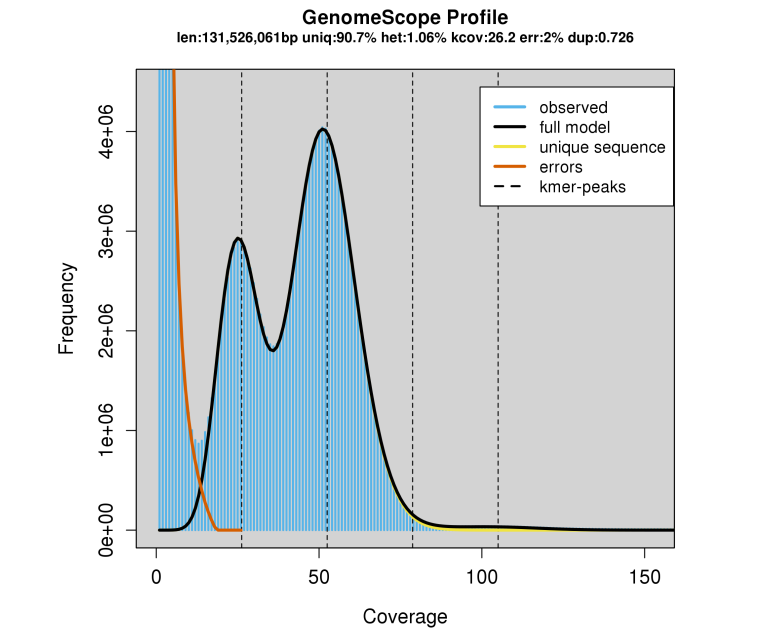
\includegraphics[width=0.6\textwidth]{capitoli/genomescope/gnmscp_genomescopeprofile.png}
		\caption{Modello del k-mer profile generato dal programma. L'istogramma in azzurro rappresenta i dati del k-mer profile reale, la curva nera il modello stimato e quella color arancione gli errori di sequenziamento stimati.}
		\label{fig:gnmscp_genomescopeprofile}
	\end{figure}


	\subsection{Gestione degli errori di sequenziamento}
	Eventuali errori di sequenziamento, ad esempio dovuti a duplicazioni con PCR o a sequenze contaminate, sono determinati solo empiricamente: dopo varie iterazioni del software in cui viene abbassata la soglia di copertura richiesta, i k-mer che non riescono ad essere rappresentati dal modello vengono identificati come errori di sequenziamento. 
	
	La stima dei k-mer sequenziati in modo errato è importante perché viene utilizzata per determinare la percentuale di basi errate nelle letture: una singola base inesatta infatti può dar luogo fino a $k$ k-mer errati, aumentando notevolmente il numero di errori. GenomeScope permette una percentuale $e$ di basi errate in ciascun k-mer. Tale valore è calcolato con un fitting dei k-mer errati a una distribuzione binomiale tramite la funzione \verb|uniroot| del linguaggio di programmazione \textit{R}. Questo metodo permette al programma di non dover assumere che la distribuzione degli errori di sequenziamento abbia una particolare forma, né di utilizzare un valore di soglia.
	
\end{document}